\chapter{Grundlagen}

\section{Projektumfeld}

Das Projekt wird im Umfeld der \gls{DHBW} Karlsruhe durchgeführt.

\section{Funktionsweise WLAN}

\subsection{SSID}

\subsection{BSSID}

\subsection{Signalstärke RSSI}

\section{Beispiel eines Workflows}

In folgender \autoref{fig:beschaffungsverfahren} ist ein Beispiel für einen Prozess an der \gls{DHBW} Karlsruhe dargestellt.
Es ist das \enquote{Beschaffungs-Genehmigungsverfahren}, das benötigt wird, um eine Bestellung für die \gls{DHBW} durchzuführen.

\begin{figure}
	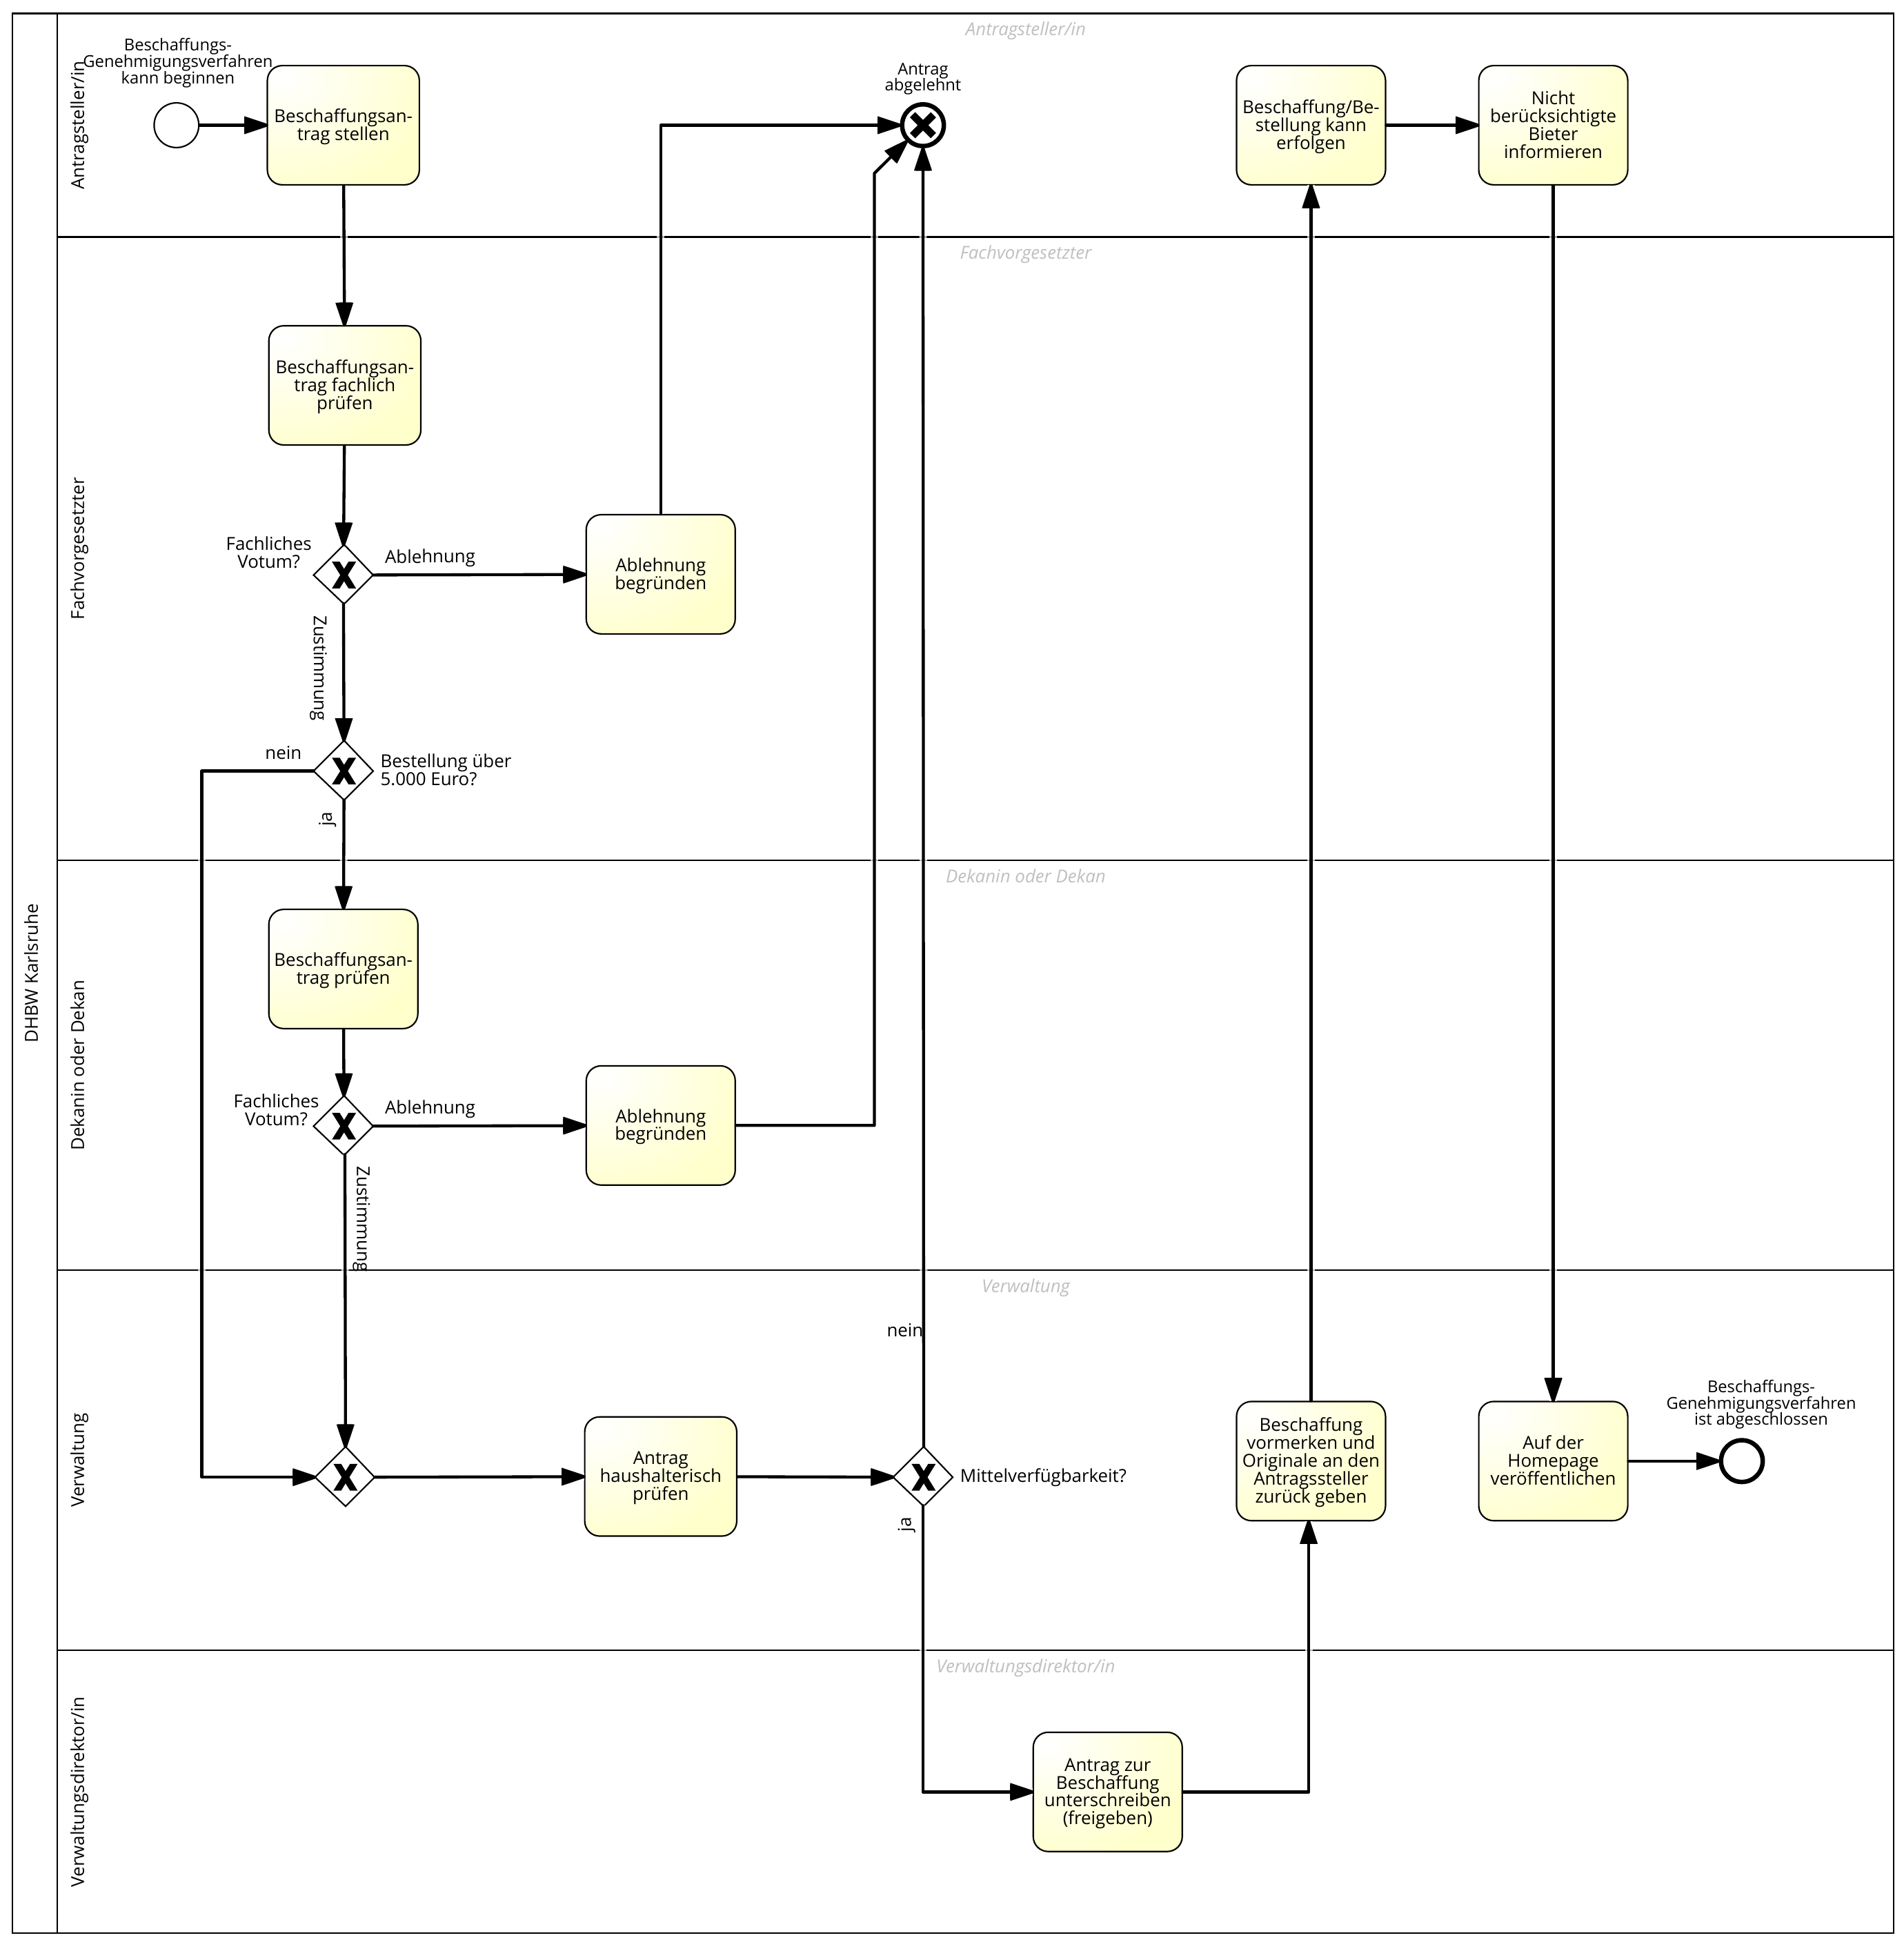
\includegraphics[width=\textwidth]{images/beschaffungs-genehmigungsverfahren.png} 
	\centering
	\caption{Beschaffungs-Genehmigungsverfahren der \gls{DHBW}}
	\label{fig:beschaffungsverfahren}
\end{figure} 

% TODO: Describe workflow
